\documentclass{article}
\usepackage[utf8]{inputenc}
\usepackage{graphicx}
\usepackage{listings}

\title{PPE Lab 2}
\author{Hannah Atmer and Xiaoyue Chen \\ Team 6}
\date{October 2021}

\begin{document}

\maketitle

\section{Performance Estimates}
Your estimates of the performance impact of the GPU offload and how you came up with them. 

\begin{figure}[h!t]
    \centering
    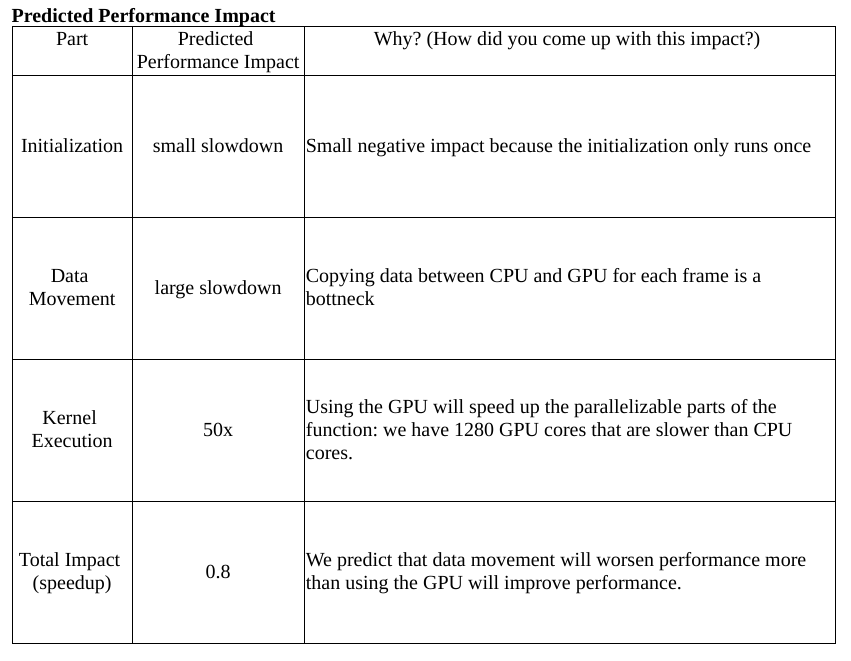
\includegraphics[width=1\textwidth]{predicted.png}
    \caption{Predicted Performance Impact}
    \label{fig:predicted}
\end{figure}

\section{Performance Achieved}

\subsection{Your measured performance results from implementing the optimizations.}

\begin{figure}[h!t]
    \centering
    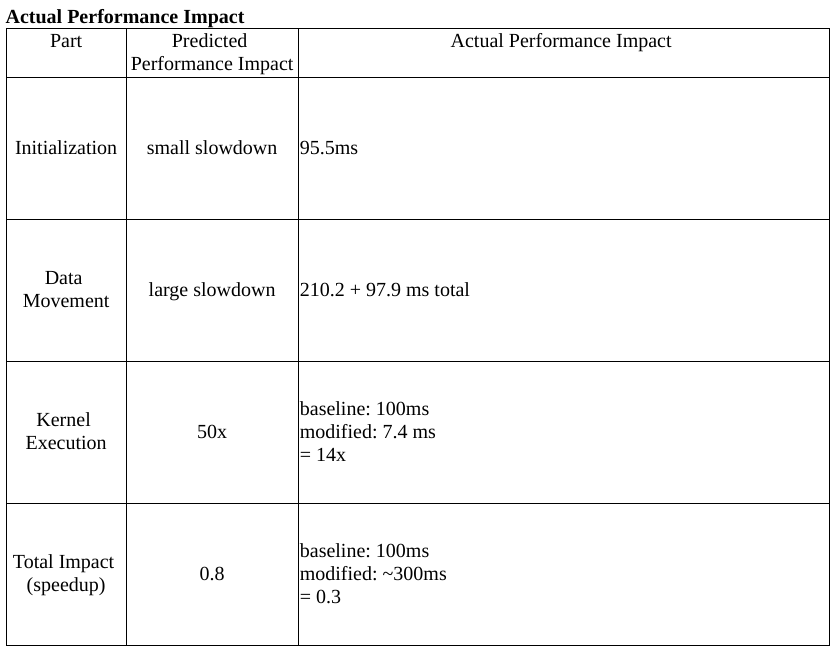
\includegraphics[width=1\textwidth]{actual.png}
    \caption{Actual Performance Impact}
    \label{fig:actual}
\end{figure}

\subsection{The parallel scaling of your implementation.}

\begin{figure}[h!t]
    \centering
    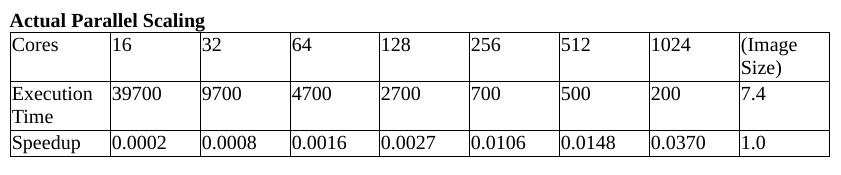
\includegraphics[width=1\textwidth]{parallel.png}
    \caption{Parallel Scaling}
    \label{fig:parallel}
\end{figure}

\section{Discussion}

\subsection{A discussion of the measured results and how they differ from your predictions.}

\subsection{A discussion of what you learned about these optimizations from implementing them and measuring the results.}

\subsection{Comment on any unexpected or odd results.}

\subsection{Comments on the difficulty of the GPU offload.}

\section{Lab comments}
Any feedback on the lab itself.

\end{document}
